One requirement of our methods specified in \ref{detectionasproofofrepresentation} is to be able
to understand the underlying representation the network ended up developing. Therefore, we present
\cite{simonyan2014deep}, which does not specifically explore counting, but will give us the tools
we need for our work.

\cite{simonyan2014deep} makes important contributions in two ways. The first is that they construct
a method by which a network can, in a sense, paint a picture that shows what the network thinks
a certain class looks like. They make the point that this method only describes the network, not
how the network comes to its conclusion on a per-sample basis. To do the latter task, they describe a method
of generating a saliency map, which we find very useful for our contributions.

In the general sense, a saliency map is an image where each pixel is given an intensity value
representing its contribution to the classification. In this paper, they work with the idea that
gradients w.r.t.\ an image is a direct saliency representation; backpropagation starts from the
desired class. The reasoning is intuitive: if the goal of a saliency map is to point out the most
salient parts of an image, then one can think of large gradients as essentially exactly what we need.
This is their method, but with a small modification: because each subpixel is assigned a gradient,
they merge the three as but there is only one value assigned to each pixel in the saliency map.
Merging consists of finding the channel with the greatest magnitude, and assign that magnitude to
the pixel for which we need to generate a value. They perform some sort of normalization as
the final values could be larger than 255 (or whatever limit the bit depth of the image implies).
Figure \ref{figure2simonyan} reproduces saliency maps that can be found in the paper.

\begin{figure}
    \begin{center}
        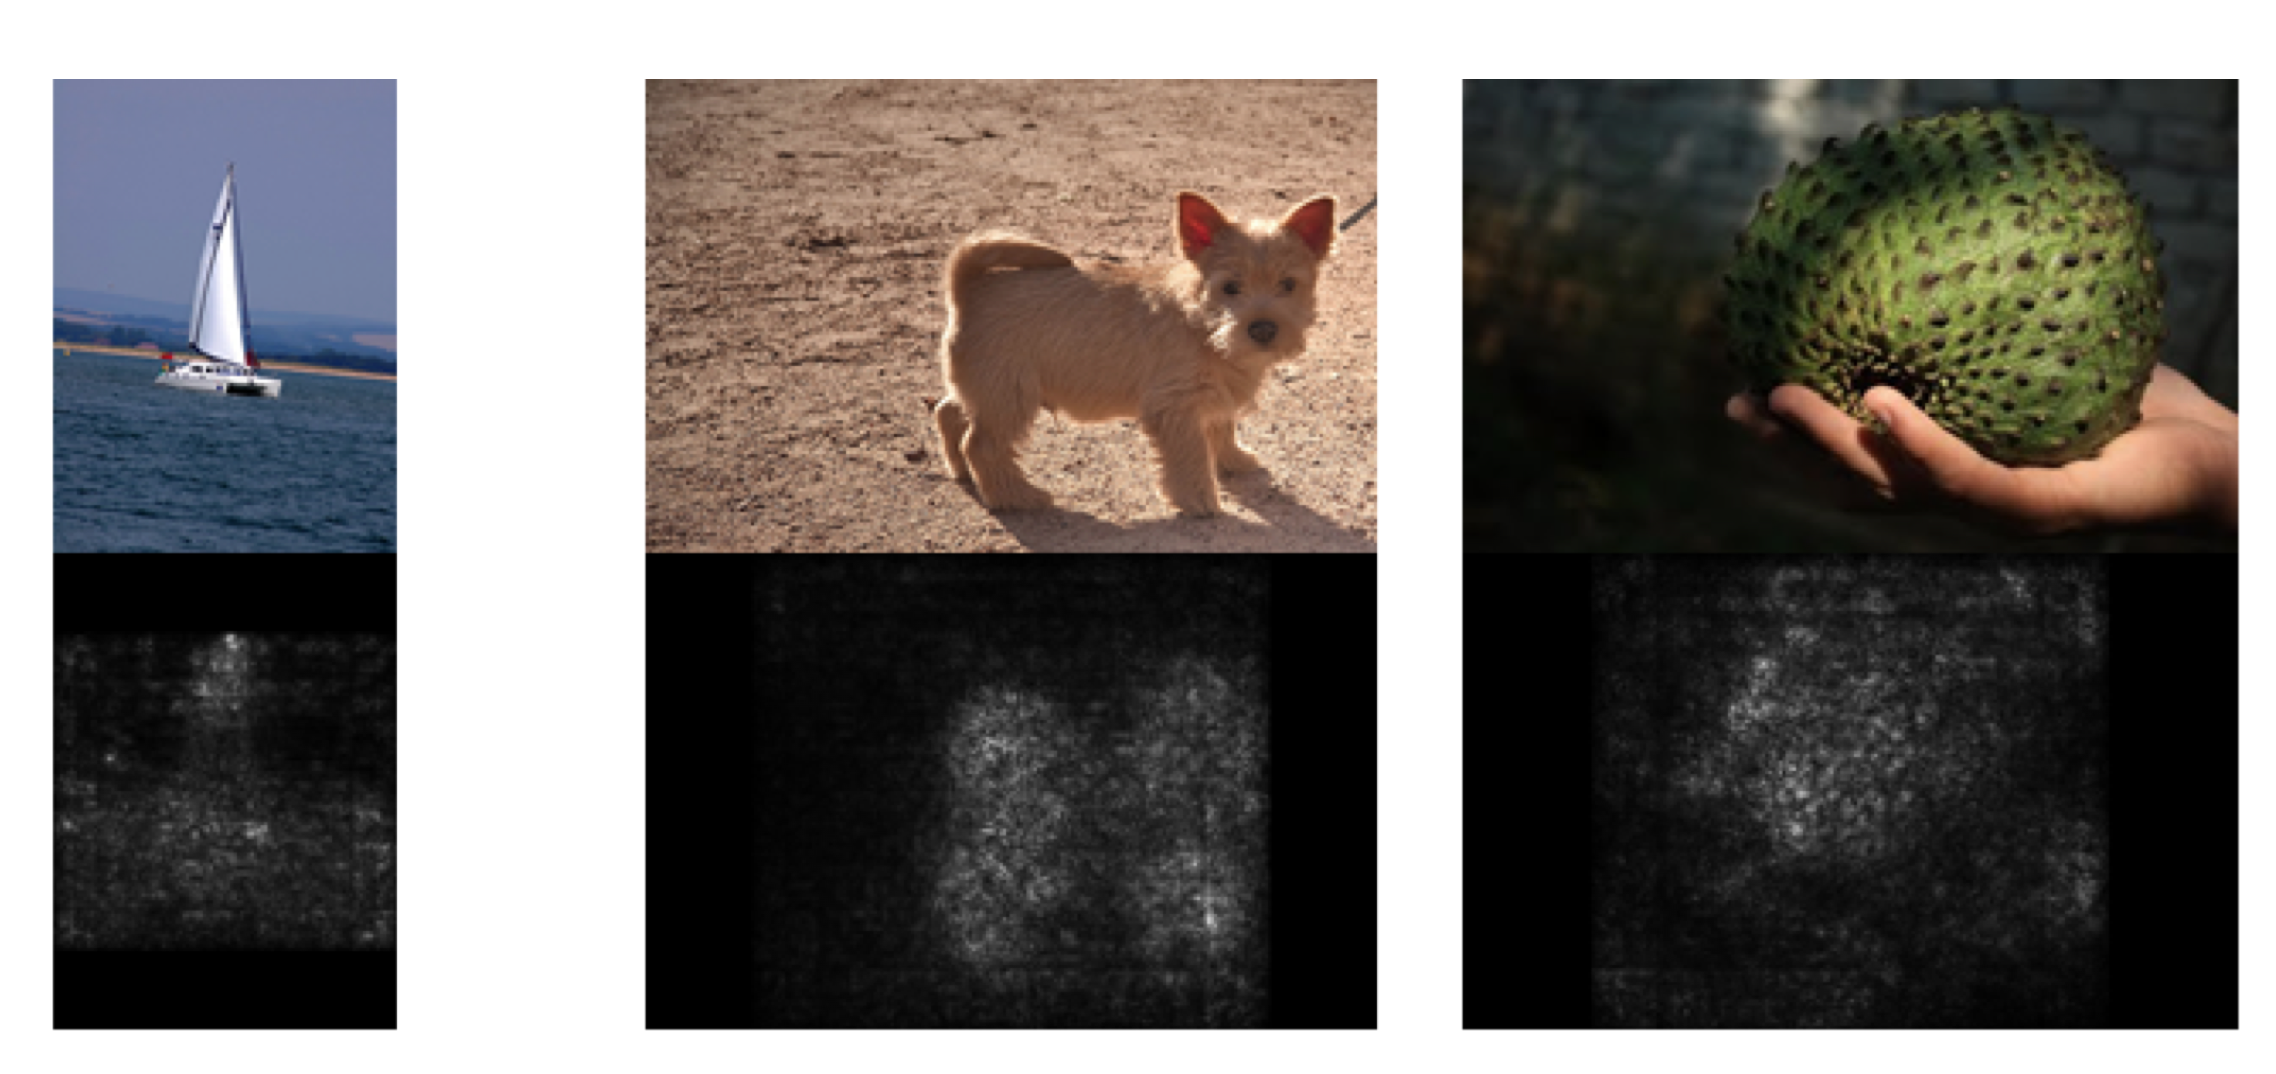
\includegraphics[width = \textwidth]{Counting/LaTeX/figures/simonyanfigure.png}
    \end{center}
    \caption{Some images and their respective saliencies they generated; from \cite{simonyan2014deep}[figure 2]}
    \label{figure2simonyan}
\end{figure}

Interestingly, they find that this saliency map can be used to determine which parts of the image
are foreground and background. This is due to the fact that the salient pixels are indications of
the foreground, and so they can be fed to an algorithm that performs the segmentation (they use
something in ~\cite{937505} to do the segmentation, but this author does not know the details of
that algorithm to elaborate how it works with the saliency map).